\let\negmedspace\undefined
\let\negthickspace\undefined
\documentclass[journal]{IEEEtran}
\usepackage[a5paper, margin=10mm, onecolumn]{geometry}
%\usepackage{lmodern} % Ensure lmodern is loaded for pdflatex
\usepackage{tfrupee} % Include tfrupee package

\setlength{\headheight}{1cm} % Set the height of the header box
\setlength{\headsep}{0mm}  % Set the distance between the header box and the top of the text

\usepackage{gvv-book}
\usepackage{gvv}
\usepackage{cite}
\usepackage{amsmath,amssymb,amsfonts,amsthm}
\usepackage{algorithmic}
\usepackage{graphicx}
\usepackage{textcomp}
\usepackage{xcolor}
\usepackage{txfonts}
\usepackage{listings}
\usepackage{enumitem}
\usepackage{mathtools}
\usepackage{gensymb}
\usepackage{comment}
\usepackage[breaklinks=true]{hyperref}
\usepackage{tkz-euclide} 
\usepackage{listings}
% \usepackage{gvv}                                        
\def\inputGnumericTable{}                                 
\usepackage[latin1]{inputenc}                                
\usepackage{color}                                            
\usepackage{array}                                            
\usepackage{longtable}                                       
\usepackage{calc}                                             
\usepackage{multirow}                                         
\usepackage{hhline}                                           
\usepackage{ifthen}                                           
\usepackage{lscape}
\begin{document}

\bibliographystyle{IEEEtran}
\vspace{3cm}

\title{1.7.11}
\author{EE24BTECH11021 - Eshan Ray}

% \maketitle
% \newpage
% \bigskip
{\let\newpage\relax\maketitle}

\renewcommand{\thefigure}{\theenumi}
\renewcommand{\thetable}{\theenumi}
\setlength{\intextsep}{10pt} % Space between text and floats




\textbf{Question: }\\
If the pair of equations $3x - y + 8 = 0$ and $6x - ry+ 16 = 0$ represent coincident lines,
then the value of $r$ is \dots\\
\solution{ Given, \begin{align}
               3x - y &= -8 \\
               6x - ry &= -16
               \end{align}
        
               So, the coefficient matrix $A = \myvec{3 & -1 \\ 6 & -r}$\\
                and the constant matrix $B = \myvec{-8 \\ -16}$
                \begin{align}
                \therefore A\vec x &= B\\
                \myvec{3 & -1 \\ 6 & -r}\myvec{x \\ y}&=\myvec{-8 \\ -16}\\
                so, \sbrak {A\mid B} &= \myvec{3 & -1 \mid & -8 \\ 6 & -r \mid & -16}
              \end{align}
              Performing row operations$\colon$ $R_2 - 2R_1\longrightarrow R_2$
              \begin{align}
            \myvec{3 & -1\mid & -8 \\ 6-\brak{2}\brak{3} & -r+\brak{2}\brak{1}\mid & -16+\brak{2}\brak{8}}=\myvec{3 & -1\mid & -8\\ 0 & -r+2\mid & 0}
              \end{align}
              For two lines to be coincident rank of matrix $\sbrak{A\mid B}$ must be $=1$
              \begin{align}
              \therefore -r+2&=0\\
              \implies r&=2
               \end{align}
 \begin{figure}[!ht]
    \centering
	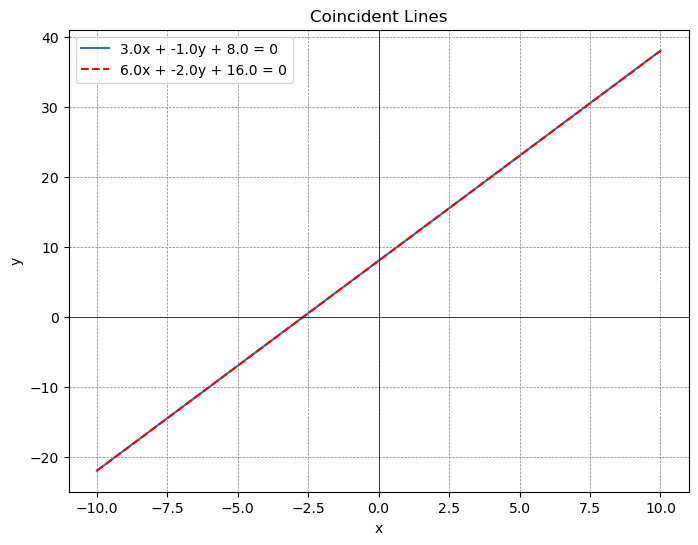
\includegraphics[width=1\textwidth]{plots/plot.png}
    \caption{Coincident Lines}
    \label{fig:plot}
\end{figure}              
}
\end{document}



 





